\section{Rappels}

\frame
{
	\frametitle{Rappels}
	Vu au cours pr\'ec\'edent :
	\begin{itemize}
		\item Historique de DICOM.
		\item DICOM est un standard, pas une norme.
		\item DICOM d\'efinit des SOP (Service-Object Pair) :
		\begin{center}
			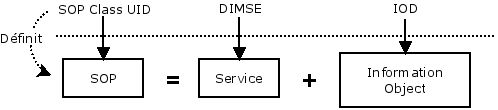
\includegraphics[width=\linewidth]{./figures/sop-definition.png}
		\end{center}
	\end{itemize}
}

\frame
{
    \frametitle{Correction des exercices}

    \begin{block}{Exercice}
        Jusqu'\`a combien pouvez-vous compter avec vos $10$ doigts ?
    \end{block}


    \begin{center}
        
\includegraphics[width=.5\linewidth]{./figures/mains.png}
    \end{center}

}

